\section{Results and Discussion}

\subsection{Single Model vs Multi Model}
\begin{figure}[H]
	\centering
	\begin{subfigure}{\textwidth}
		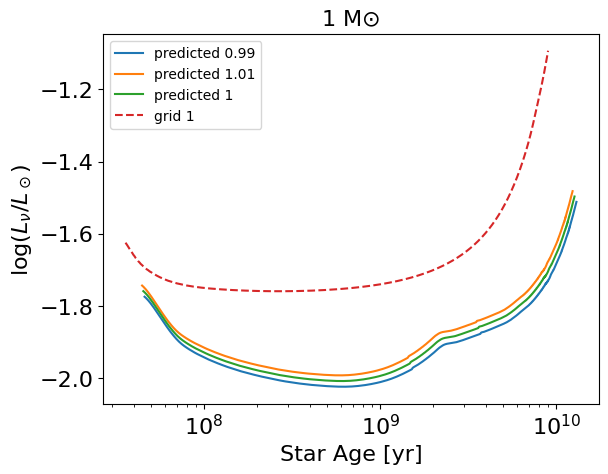
\includegraphics[width=\textwidth,height=0.5\textheight]{assets/output1singlemodel.png}
		\caption{Sun $1M\odot$ Single Testing Data.}
		\label{fig:SunTesta}	
	\end{subfigure}
	\begin{subfigure}{\textwidth}
		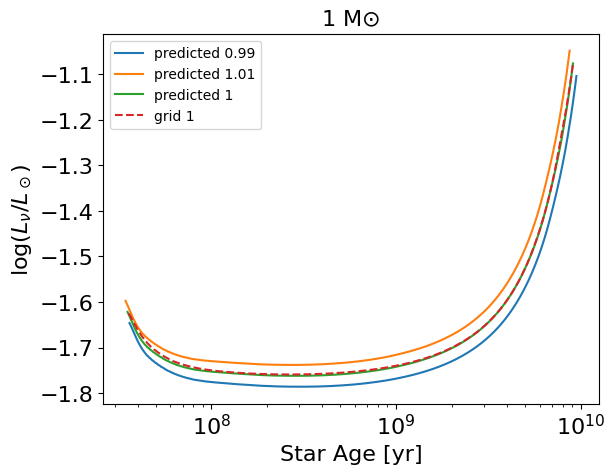
\includegraphics[width=\textwidth,height=0.5\textheight]{assets/output1.png}
		\caption{Sun $1M\odot$ Multi Model($0.5-1.1M_\odot$) Testing Data.}
		\label{fig:SunTestb}	
	\end{subfigure}
	\caption{Prediction Model testing grid $1M_\odot$}
	\label{fig:SunTest}
\end{figure}


\begin{figure}[H]
	\centering
	\begin{subfigure}{\textwidth}
		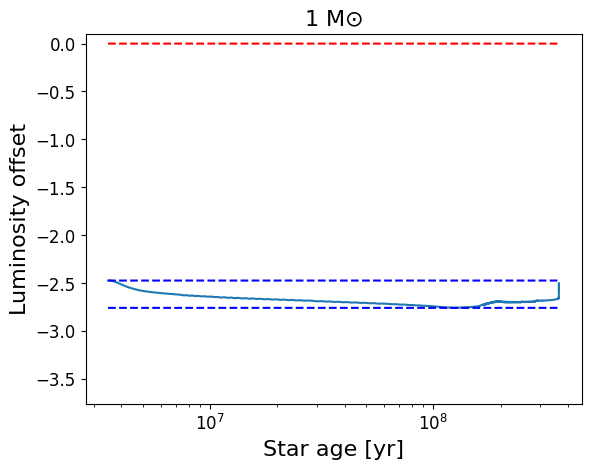
\includegraphics[width=\textwidth,height=0.5\textheight]{assets/error1modelsingle.png}
		\caption{Luminosity Offset for $1M\odot$.}
	\end{subfigure}
	\begin{subfigure}{\textwidth}
		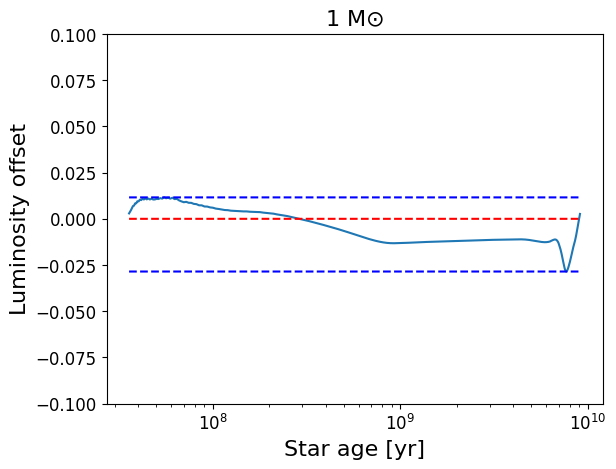
\includegraphics[width=\textwidth,height=0.5\textheight]{assets/error 1.png}
		\caption{Multimodel Error for $1M\odot$.}	
	\end{subfigure}
	\caption{Comparison of Luminosity offset for Single Model and Multi Model($0.5-1.1M_\odot$) for $1M_\odot$}
	\label{fig:lumoff}
\end{figure}

\begin{figure}[H]
	\begin{subfigure}{\textwidth}
		\centering
		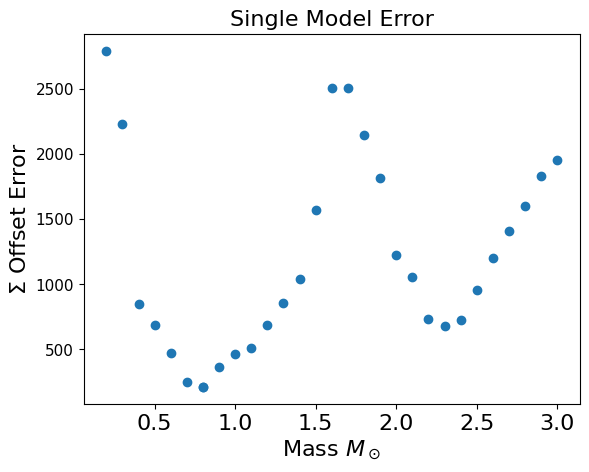
\includegraphics[width=\textwidth,height=0.5\textheight]{assets/singlemodeerror.png}
		\caption{Single Model Error.}
		\label{fig:sumerrorsinglea}
	\end{subfigure}
	\begin{subfigure}{\textwidth}
		\centering
		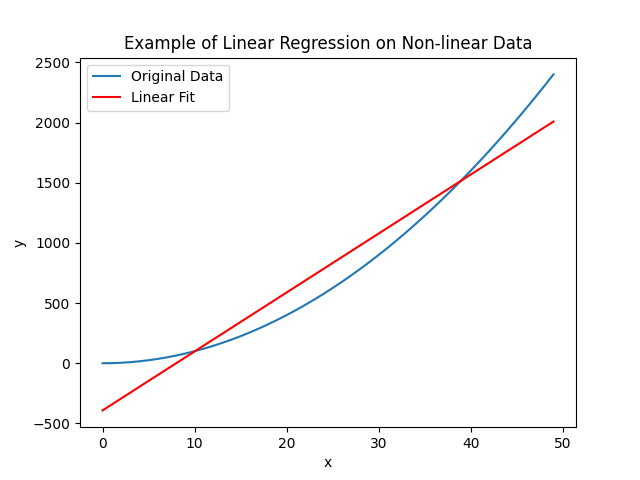
\includegraphics[width=\textwidth,height=0.5\textheight]{assets/Examplenonlinreg.png}
		\caption{Example of Linear Regression on Non-linear data.}
		\label{fig:sumerrorsingleb}
	\end{subfigure}
	\caption{Sum offset error for single model.}
	\label{fig:sumerrorsingle}
\end{figure}


\begin{figure}[H]
	\begin{subfigure}{\textwidth}
		\centering
		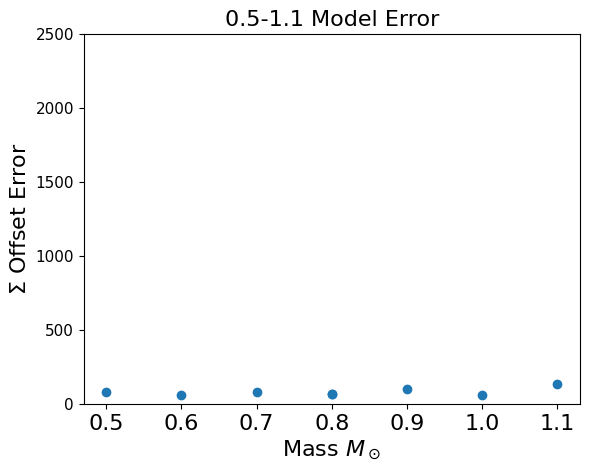
\includegraphics[width=\textwidth,height=0.5\textheight]{assets/0.5-1.1Error.png}
		\caption{$0.5-1.1M\odot$ Model Error.}
		\label{fig:sumerrormultia}
	\end{subfigure}
	\begin{subfigure}{\textwidth}
		\centering
		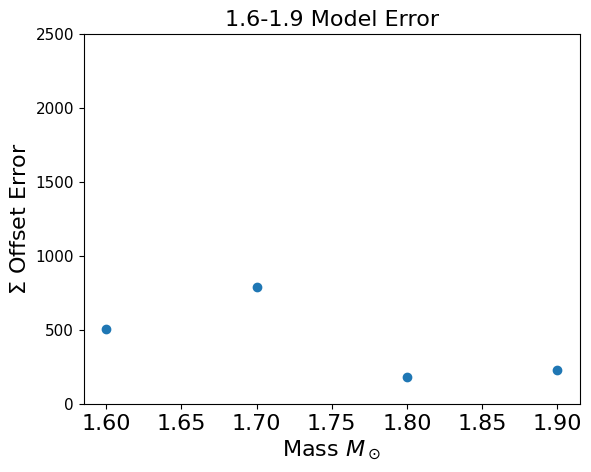
\includegraphics[width=\textwidth,height=0.5\textheight]{assets/1.6-1.9error.png}
		\caption{$1.6-1.9M\odot$ Model Error.}
		\label{fig:sumerrormultib}
	\end{subfigure}
	\caption{Sum offset error for multi model.}
	\label{fig:sumerrormulti}
\end{figure}

Figure~\ref{fig:SunTest} Was both plotted from different model where a is using a single model meaning the linear regression was done using all the data as one model and b is done using multi model meaning that the data is separated into section and linear regression was done on each section separately, for this case the model for $0.5-1.1 M_\odot$. These plots are made by removing $1M_\odot$ from the grid to be used as testing data. We can see that for the single model prediction that it is very deviated from the grid and the shape is different from the grid and the multi model prediction strongly follows the $1M_\odot$ grid.

The luminosity offset between the 1Mo prediction and 1Mo grid is then calculated and plotted on Figure~\ref{fig:lumoff}. The single model has the smallest offset of around -2.47 and a highest offset of -2.76. The multi model has an upper bound offset of 0.02 and a lower bound of -0.03. From these values we can say that the single model is heavily biased to the negative side and has around 250\% error while the multi model has no bias since the offset is balanced and has around 2\% error. 

This was done across for all the masses for all models as example shown in Figure~\ref{fig:sumerrorsinglea}, \ref{fig:sumerrormultia}, and \ref{fig:sumerrormultib}. However for this plot instead of just calculating the luminosity offset, Formula~\ref{Eq:er} was used in order to calculate the total offset from datapoint to datapoint meaning accounting both luminosity and star age. The show was done using a single model and we can see the error fluctuates quite a lot. This actually indicates that the data is not linear, and after taking a look at the 3D plot Figure~\ref{fig:3dplt}, we see that the data have a sort of exponential shape. We can see from the Figure~\ref{fig:sumerrorsingleb} as an example where when linear regression is done on a non linear data we can see that the error will be small when the linear fit intercept with the line. However, other than that the error would be huge just like in Figure~\ref{fig:sumerrorsinglea} In order to account for this that is why we decided to section the data in order to minimize the error due to the non linearity of the data.

After doing the same analysis on the multi model, we get around the same shape as Figure~\ref{fig:sumerrormultia}, however when done using the 1.6-1.9 model there is a sudden rise in error. If we look at the data used in this model, we can see that there is large variation especially in the tail section of the plot as seen in Figure~\ref{fig:1.6-1.9}. If this variation relates to the real physical variation during stellar evolution we truly cannot use linear regression for this section. The other possibility is that this variation came from artefact, if this is true then we can apply smoothing/outlier removal before doing the linear regression in order to account for this.

\subsection{Prediction of Flux}

\begin{table}[H]
    \centering
	\caption{Stars with their mass and distance.}
	\label{tab:stars and mass}
	\begin{tabular}{ccc}
		\toprule
		Star & Mass [$M\odot$]  & Distance [$pc$] \\
		\midrule
		Sun & $1$ & $4.85\times 10^{-6}$\\
		$\tau$ ceti & $0.78$ & $3.65$\\
		Sirius & $2.06$ & $2.64 $\\
		\bottomrule
	\end{tabular}
\end{table}
\begin{figure}[H]
	\centering
	\begin{subfigure}{\textwidth}
		\centering
		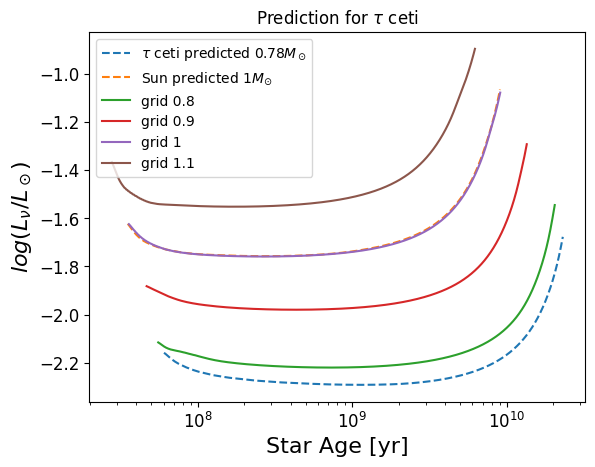
\includegraphics[width=\textwidth,height=0.5\textheight]{assets/predtauceti.png}
		\caption{Prediction for $\tau$ ceti $0.78 M\odot$.}
		\label{fig:tau}	
	\end{subfigure}
	\begin{subfigure}{\textwidth}
		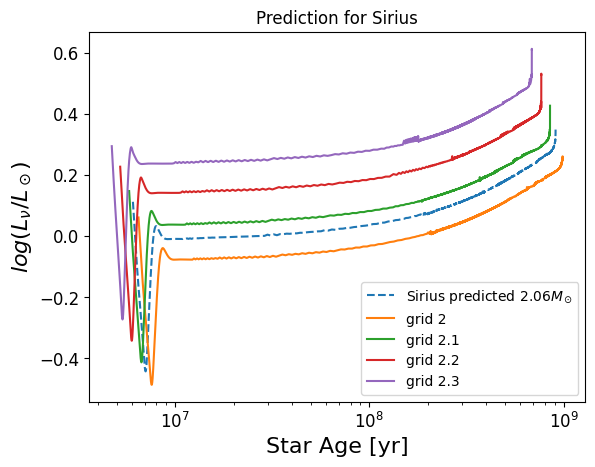
\includegraphics[width=\textwidth,height=0.5\textheight]{assets/predsirius.png}
		\caption{Prediction for Sirius $2.06 M\odot$.}
		\label{fig:Sirius}
	\end{subfigure}
	\caption(Prediction of different Stars Luminosity and Ages Using Multi Model)
	\label{fig:predict}
\end{figure}            
\begin{figure}[H]

\end{figure}

\begin{figure}[H]
	\centering
	\begin{subfigure}{\textwidth}
		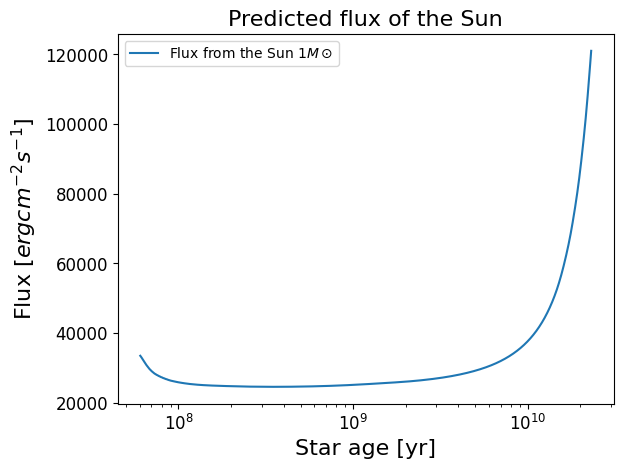
\includegraphics[width=\textwidth,height=0.5\textheight]{assets/fluxsun.png}
		\caption{Prediction for Flux of Sun $1 M\odot$.}
	\end{subfigure}
	\begin{subfigure}{\textwidth}
		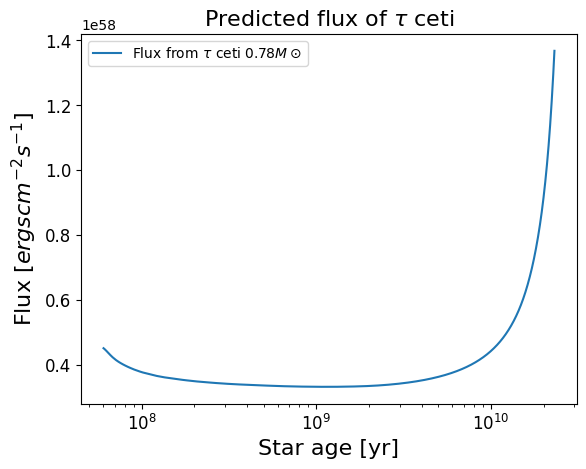
\includegraphics[width=\textwidth,height=0.5\textheight]{assets/fluxtau.png}
		\caption{Prediction for flux of $\tau$ ceti $0.78 M\odot$.}
	\end{subfigure}
	\begin{subfigure}{\textwidth}
		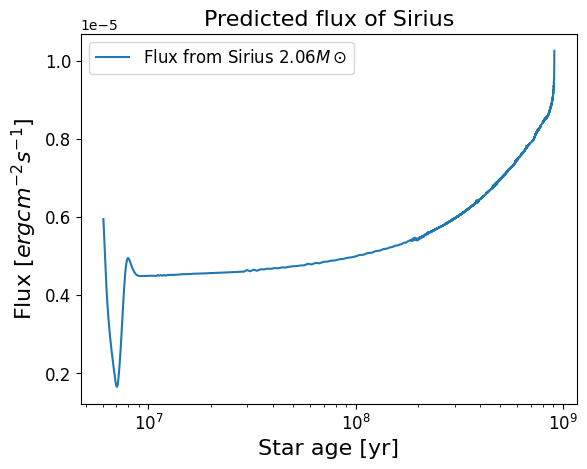
\includegraphics[width=\textwidth,height=0.5\textheight]{assets/fluxsirius.png}
		\caption{Prediction for flux of Sirius $2.06 M\odot$.}
	\end{subfigure}
	\caption(Flux Prediction)
	\label{fig:predicted flux}
\end{figure}

We then decide to use the multi model for prediction of flux from distant stars. We used the data in Table~\ref{tab:stars and mass} to predict flux coming from the Sun and $\tau$ ceti where the mass is the mass of the star in term of solar mass and the distance is the distance between the earth and the stars. Figure~\ref{fig:tau} shows plots of $log(l_\nu/l_\odot)$(where $l_\odot=3.828\times 10^33ergs^-1$ prediction for t ceti and sun and part of the grid of the model training for comparison. We can see that for the $\tau$ ceti with mass $0.78M_\odot$ it is where we expect it to be, which is below grid 8 and for the sun, it is the same as in Figure~\ref{fig:SunTestb}. The same can be said Sirius with mass of $2.06M_\odot$ where it is between grid 2 and 2.1. Using the prediction data we then calculate the flux for both the Sun, Sirius and $\tau$ ceti as seen in Figure~\ref{fig:predicted flux} The prediction shows that the flux coming from the sun is of 12 orders of magnitude compared to flux coming from tau ceti. When the fluxes are plotted together, the flux of $\tau$ ceti will look like it is non-existence. Though Sirius is 2 times more massive than the sun and producing more neutrino, due to the massive different in distance it the neutrino flux on earth are still small by 9 order of magnitude. This is the reason why it is so hard to detect the neutrino coming from these distant stars. 

From this we can see that linear regression can be used but it is not the best method. Even after sectioning the data, when met with data that contains huge variation it tends to fail as linear regression is very sensitive to outliers. This means that an even better method needs to be tested, especially one that can handle non-linear data especially in order to incorporate the helium burning stage into the training data in order to predict the neutrino flux coming from that stage of the star's evolution. Methods that can be tested out are neural networks as it is capable of capturing complex patterns in highly non-linear data and may be able to create a more accurate prediction model.

For further testing, cross-validation can be applied to assess model robustness across different data splits, while testing with various data subsets, especially focusing on distinct mass ranges or evolutionary stages, can provide more targeted validation. Incorporating additional astrophysical parameters, such as metallicity or temperature, may capture more variability and improve the model's accuracy. To enhance model performance, strategies like smoothing techniques can reduce noise, and outlier removal can mitigate the impact of anomalous points. Feature engineering can create new, more informative variables, and using model ensembles can balance predictions by leveraging the strengths of multiple models.
